\documentclass[bluish,slideColor,colorBG]{prosper}
\hypersetup{pdfpagemode=FullScreen}
\usepackage{graphicx}
\def\baselinestretch{0.7}
\setlength{\topmargin}{-60pt}
\setlength{\textheight}{700pt}
\setlength{\oddsidemargin}{0pt}
\setlength{\evensidemargin}{60pt}
\setlength{\textwidth}{477pt}
\setlength{\footskip}{0pt}
\parindent 0.3in
\hyphenpenalty=10000
\tolerance=10000
\pagestyle{empty}

\title{Week 9}
\author{Joe Felsenstein}
\institution{Genome 562, 2017}

\begin{document}

{\parindent=0in

\maketitle

\begin{slide}[Replace]{Effect of a bottleck on effective number}

\centerline{
\begin{tabular}{c c c c}
\multicolumn{2}{c}{Number of generations at:} & \multicolumn{2}{c}{Effective
pop
ulation number}\\
$N_i  =  10$     &       $N_i  =  1000$        &           $N_e$ (approximate)  
&      $N_e$ (exact)\\
\hline
1       &           99          &                 502.51       &
496.25\\
5        &          95           &                168.07       &
164.74\\
10       &           90          &                  91.74      &
89.86
\\
25       &           75          &                  38.83      &
38.13
\\
50       &           50          &                  19.80      &
19.56
\\
75       &           25          &                  13.29      &
13.21
\\
90       &           10          &                  11.10      &
11.07
\\
99       &            1          &                  10.10      &
10.10
\end{tabular}
}

\end{slide}

\begin{slide}[Replace]{Views of genetic variation before 1966}

\begin{tabular}{c c}
The Classical view  & The Balancing Selection view \\
\includegraphics[width=1in]{muller.ps} & \includegraphics[width=1.2in]{dobybrazil.ps} \\
Hermann Joseph Muller & Theodosius Dobzhansky \\
 & \\
Most loci will be homozygous   &    Most loci will be polymorphic \\
for the ``wild-type allele"    &    due to balancing selection \\
but a few mutants will exist   &    with strong selection \\
\end{tabular}

\noindent

\end{slide}

\begin{slide}[Replace]{Polymorphism on a gel}

\centerline{\includegraphics[width=4in]{gelpoly.ps}}

\end{slide}

\begin{slide}[Replace]{Lewontin and Hubby's 1966 work}

\centerline{
\includegraphics[width=1.5in]{lewontin.ps}}

\noindent
\centerline{Richard Lewontin, about 1980}
\bigskip

\noindent
Lewontin, R. C.  and J. L. Hubby.  1966.  A molecular approach to the study of genic heterozygosity in natural populations. II. Amount of variation and degree of heterozygosity in natural populations of Drosophila pseudoobscura.
{\it Genetics} {\bf 54:} 595-609.

\end{slide}

\begin{slide}[Replace]{Neutral mutation theory}

\hspace*{0in} \hfill 
\includegraphics[width=2.3in]{CrowKimura72sm.ps} \hfill 
\includegraphics[width=1.07in]{ohta.ps} \hfill  {~~}

~~~~~~~~ James F. Crow and Motoo Kimura, 1972 ~~~~ Tomoko Ohta, recently
\bigskip

{\parindent=-15pt
Kimura, M., and J. F. Crow. 1964.  The number of alleles that can be maintained in a finite population. {\it Genetics} {\bf 49:} 725-738.

Kimura, M. 1968. Evolutionary rate at the molecular level. {\it Nature}
{\bf 217:} 624-626.

Kimura, M.,  and T. Ohta.  1971.  Protein polymorphism as a phase of molecular
e8volution. {\it Nature} {\bf 229:} 467-469.
}

\end{slide}

\begin{slide}[Replace]{DNA sequencing reveals a similar picture}

\noindent
\centerline{
\includegraphics[width=1in]{kreitman2.ps}}

\noindent
\centerline{Marty Kreitman}
\bigskip

\noindent
Kreitman, M. 1983. Nucleotide polymorphism at the alcohol-dehydrogenase Locus
 of {\it Drosophila melanogaster}. {\it Nature} {\bf 304:} 412-417.


\end{slide}

\begin{slide}[Replace]{Kreitman's sample of 11 ADH gene sequences, front end}

\noindent
\centerline{\includegraphics[width=3.5in]{kreitmanexpt1.ps}}
\centerline{\includegraphics[width=3in]{kreitmanexpt3.ps}}

\end{slide}

\begin{slide}[Replace]{Kreitman's sample of 11 ADH gene sequences, tail end}

\noindent
\centerline{\includegraphics[width=3.5in]{kreitmanexpt2.ps}}
\centerline{\includegraphics[width=3in]{kreitmanexpt3.ps}}

\end{slide}

\begin{slide}[Replace]{Individual alleles do not stay at an equilibrium}
\bigskip

\centerline{\includegraphics[width=3in]{neutral.idraw}}

\end{slide}
}

\end{document}

